\section{LTE 네트워크의 구성 요소}
% \vspace{-4mm}  
% \begin{figure}[!h]\centering
% 	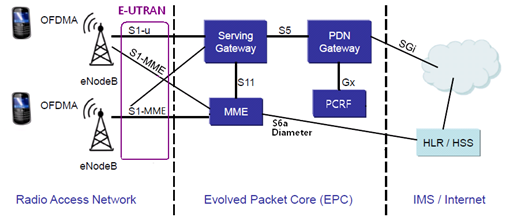
\includegraphics[width=.7\textwidth]{image/week11/1-1.png}
% 	\caption{\small LTE Network Structure}
% 	\vspace{-10pt}
% \end{figure}
\vspace{-4mm}  
\begin{figure}[!h]\centering
	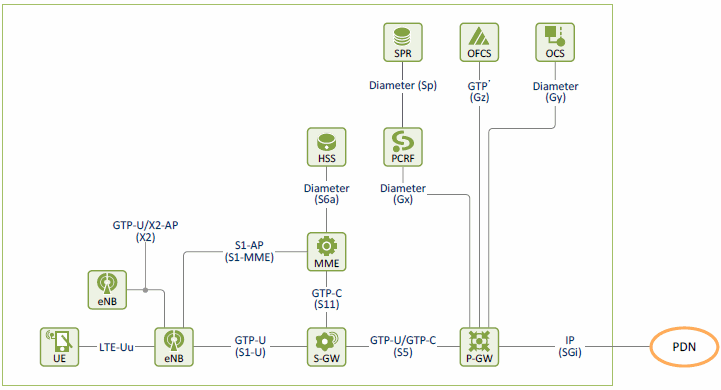
\includegraphics[width=.7\textwidth]{image/week11/1-2.png}
	\caption{\small LTE Network Components}
	\vspace{-10pt}
\end{figure}
LTE(Long Term Evolution)는 OFDM, MIMO, SDR 등의 고속 패킷 전송에 최적화된 기술들을 바탕으로 한 4세대 이동통신 기술이다. 위의 그림은 LTE 네트워크의 구조를 도식화 한 것이다. LTE 네트워크는 eNodeB로 구성된 무선 접속망인 RAN(Radio Access Network)와 MME, S-GW, P-GW, HSS 등으로 구성된 Core 망인 EPC(Evolved Packet Core)로 나누어 지고, 이 둘을 통합하여 EPS(Evolved Packet System)이라고 부른다. \\
LTE 네트워크의 구성요소는 다음과 같다.

    \subsubsection*{UE (User Equipment)}
    사용자 단말이다. 가입자 식별/인증을 위한 IMSI(International Mobile Station Identity, 국제 이동국 식별번호)값이 내장된 USIM  카드를 삽입할 수 있다. 내장된 LTE chip으로 LTE 망에 접속할 수 있다.
\vspace{-2mm}
    \subsubsection*{eNodeB (Evolved Node B)}
    LTE 기지국이다. UE와 LTE 네트워크 간에 무선 연결을 제공한다. UE와 eNodeB는 무선 연결되어 있고, 나머지는 IP를 통한 유선 연결이다.
\vspace{-2mm}
    \subsubsection*{E-UTRAN (Evolved Universal Terrestrial Radio Access Network)}
    LTE eNodeB로 구성된 무선 접속망이다. IP 기반의 flat한 구조로 UE와 CN(Core Network간의 데이터를 처리한다.
\vspace{-2mm}
    \subsubsection*{S-GW (Serving Gateway)}
    UE 이동으로 eNodeB간의 handover 발생 시 anchor point 역할을 한다.
\vspace{-2mm}
    \subsubsection*{P-GW (Packet data network Gateway)}
    P-GW의 역할은 다음과 같다.
    \begin{enumerate}
        \item UE에 IP 주소를 할당한다.    \vspace{-1mm}
        \item S-GW들에 대한 anchoring을 수행한다. \vspace{-1mm}
        \item UE별로 서로 다른 QoS(Quality of Service) 정책을 적용한다. (우선 순위, 대역폭 제어 등) \vspace{-1mm}
        \item UE별로 Accounting Data(트래픽 양, 접속 시간 등)을 관리한다. Accounting Data는 CDR(Charging Data Record)의 형태로 OFCS에 전달된다. \vspace{-1mm}
    \end{enumerate}
\vspace{-2mm}
    \subsubsection*{MME (Mobility Management Entity)}
    LTE 네트워크의 두뇌 역할을 하는 장비로, 역할은 다음과 같다.
    \begin{enumerate}
        \item UE를 인증(Authentication)한다. 인증 프로토콜로 EPS-AKA를 사용하고, 인증의 Key 정보를 HSS로부터 받아와 UE 인증을 수행한다.    \vspace{-1mm}
        \item EPS 베리어({UE - eNB - S-GW - P-GW} 구간에서 생성되는 논리 터널(GTP 터널))을 관리한다. MME는 EPS 베리어를 생성/변경/해제 등을 수행한다. \vspace{-1mm}
        \item 가입자의 Mobility 상태(현재 UE가 LTE 망에 연결되어 있는지, 연결되지 않았는지, 연결되고 있는데 인터넷을 사용하는지 아니면 사용하고 있는 않은지(Idle state))를 관리한다. \vspace{-1mm}
    \end{enumerate}
\vspace{-2mm}
    \subsubsection*{HSS (Home Subscriber Server)}
    UE 인증에 필요한 Key 정보와 가입자 프로필을 가지고 있는 LTE 망의 중앙 data base이다. 가입자 프로필에는 각 가입자가 가입한 서비스 상품에 맞는 QoS 등급 정보(우선 순위, 최대 사용 가능 대역폭 등)가 들어있다. 인증 Key 정보와 가입자 프로필은 UE가 LTE 망에 접속할 때 HSS에서 MME로 전달된다.
\vspace{-2mm}
    \subsubsection*{PCRF (Policy and Charging Rule Function)}
    UE별로 정책(Policy)과 과금(Charging)에 대한 Rule을 정하는 장비이다. 정책은 UE가 사용할 QoS 정보이고, 과금은 Offline 과금을 할 것인지, Online 과금을 할 것인지에 대한 정보이다. 이 정보들은 PCRF에서 P-GW로 전달되어 UE에 대한 QoS와 Charging을 수행한다.
\vspace{-2mm}
    \subsubsection*{SPR (Subscriber Profile Repository)}
    각 UE의 Policy 및 Charging Rule(Access Profile)은 SPR이라는 data base에 저장되어 있고, SPR은 PCRF에게 Access Profile을 전달한다.
\vspace{-2mm}
    \subsubsection*{OCS (Online Charging System)}
    선불제(Prepaid)를 사용하는 통신사업자들이 이용하는 과금 시스템이다. 예를 들어, 한달 동안 2GB 사용 가능한 선불카드를 구매한 가입자에 대하여, 데이터 사용량을 실시간으로 관리하다가 2GB를 다 소모한 시점(혹은 한 달이 지난 시점)에 사용자가 더 이상 인터넷을 사용하지 못하도록 한다. \\
    실시간 데이터 사용량은 P-GW에서 관리하고 그 정보를 OCS가 받아 사용자별로 남은 사용량(balance 혹은 credit)을 중앙 관리하고 credit을 다 사용한 가입자를 판별하여 더 이상 인터넷을 사용하지 못하도록 P-GW에 정보를 전달한다.
\vspace{-2mm}
    \subsubsection*{OFCS (Offline Charging System)}
    P-GW가 전달해 주는 CDR(Charging Data Record)을 받아 중앙 관리하는 장비이다.
\vspace{-2mm}
    \subsubsection*{PDN (Packet Data Network)}
    PDN = Internet = IP Network
\newpage
